\documentclass[tikz,border=3pt]{standalone}
\usepackage[utf8]{inputenc}
\usepackage[T1]{fontenc}
\usepackage{lmodern}
\renewcommand{\familydefault}{\sfdefault}
\usepackage{sansmath}\sansmath
\usepackage{chemfig}
\usepackage{pgfplots}\pgfplotsset{compat=1.18,/pgf/number format/use comma,/pgf/number format/1000 sep={.}}
\usetikzlibrary{arrows.meta,calc,positioning,decorations.pathmorphing,patterns}
% paleta del sitio
\definecolor{nar}{HTML}{E8680C}\definecolor{narc}{HTML}{FFB35C}\definecolor{hielo}{HTML}{FFF3E8}
\definecolor{tinta}{HTML}{1D1D1F}\definecolor{gris}{HTML}{6E6E73}\definecolor{lila}{HTML}{7C5CF0}
\definecolor{azul}{HTML}{2F6FD6}\definecolor{menta}{HTML}{17A673}\definecolor{coral}{HTML}{E8342A}
\begin{document}
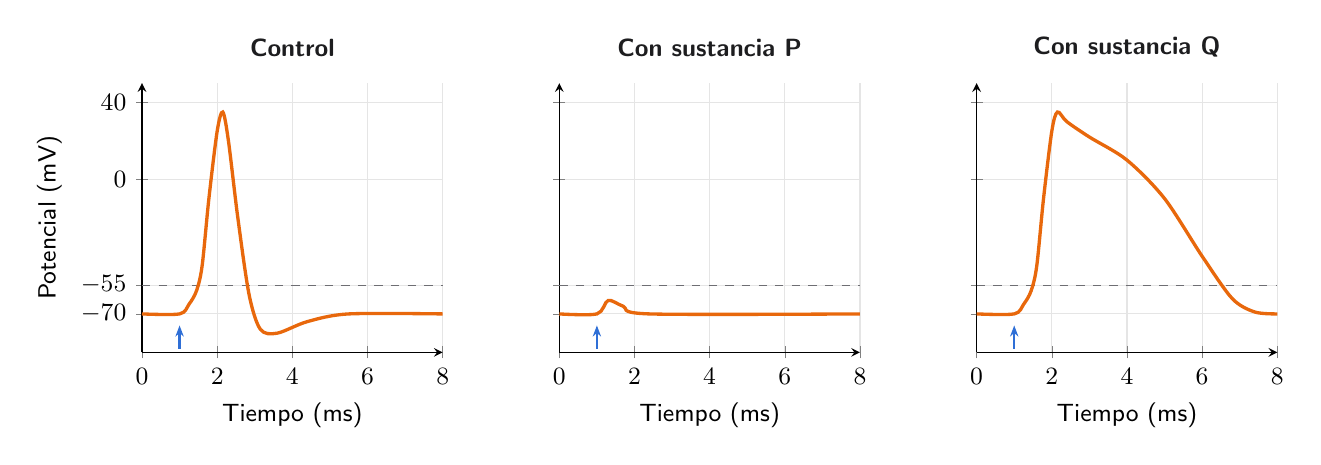
\begin{tikzpicture}[font=\small]
\pgfplotsset{mini/.style={width=5.4cm,height=5cm,axis lines=left,grid=major,grid style={gray!20},xmin=0,xmax=8,ymin=-90,ymax=50,
  xtick={0,2,...,8},ytick={-70,-55,0,40},title style={font=\small\bfseries,text=tinta},xlabel={Tiempo (ms)},clip=false}}
\begin{axis}[mini,title={Control},ylabel={Potencial (mV)},at={(0,0)}]
\addplot[gris,dashed,domain=0:8] {-55};
\addplot[nar,very thick,smooth,tension=0.5] coordinates {(0,-70)(1,-70)(1.25,-65)(1.45,-58)(1.6,-45)(1.78,-10)(2.0,25)(2.15,35)(2.3,20)(2.55,-20)(2.85,-60)(3.15,-78)(3.6,-80)(4.4,-74)(5.5,-70)(8,-70)};
\draw[-{Stealth[length=4pt]},azul,thick] (axis cs:1,-88) -- (axis cs:1,-76);
\end{axis}
\begin{axis}[mini,title={Con sustancia P},at={(5.3cm,0)},yticklabels={}]
\addplot[gris,dashed,domain=0:8] {-55};
\addplot[nar,very thick,smooth,tension=0.5] coordinates {(0,-70)(1,-70)(1.3,-63)(1.7,-66)(2.4,-70)(8,-70)};
\draw[-{Stealth[length=4pt]},azul,thick] (axis cs:1,-88) -- (axis cs:1,-76);
\end{axis}
\begin{axis}[mini,title={Con sustancia Q},at={(10.6cm,0)},yticklabels={}]
\addplot[gris,dashed,domain=0:8] {-55};
\addplot[nar,very thick,smooth,tension=0.5] coordinates {(0,-70)(1,-70)(1.25,-65)(1.45,-58)(1.6,-45)(1.78,-10)(2.0,25)(2.15,35)(2.4,30)(3,22)(4,10)(5,-10)(6,-40)(6.8,-62)(7.4,-69)(8,-70)};
\draw[-{Stealth[length=4pt]},azul,thick] (axis cs:1,-88) -- (axis cs:1,-76);
\end{axis}
\end{tikzpicture}
\end{document}
